
\section{Question 2}
\label{part2}
\begin{itemize} 
\item Ingest the 100 URIs from their resulting WARC files into a SOLR instance
	   - see the code + tutorial at:
	    ``\url{https://github.com/ukwa/webarchive-discovery}''

\item Demonstrate several functioning queries on the files(a full front-end is not required)
	  - describe the configuration choices you made in setting up SOLR and processing the 
	  	documents
\end{itemize}

\subsection{Solution}

The following steps were taken to configure SOLR and process documents :
\begin{itemize}
	\item The pre-requisites for SOLR are Maven 3, Java 7 so I installed them.
	\item I faced an issue while installing SOLR which is jetty dependency not found.
	\item I got it working by adding the dependency to the pom.xml
	\item The command ``mvn jetty:run-exploded'' starts the SOLR instance.
	\item I indexed the WARC file by using the command ``java -jar path of jar -s ``\url{http://localhost:8080/discovery}'' -t Path of WARC''.
	\item I tried to set-up Shine for SOLR as the front end instead of the default UI for SOLR but after trying for two days and multiple email exchanges with the author of the tool I wasn't able to. So I used the default SOLR front end.
	\item In SOLR we can perform the following queries.
	\begin{itemize}
	\item Here we are demonstrating how to retrieve the names and ids of all documents with ``\url{http://localhost:8080/solr/select?q=inStock:false&wt=json&fl=id,name}''
	\item Here we are using the functional query idf(field,term). This function returns the inverse document frequency for the given term, using the similarity for the field. ``\url{http://localhost:8080/solr/select/?fl=score,id&defType=func&q=mul(tf(text,memory),idf(text,memory))}''
	
	\item The functional query being used here is tf(field,term) and it returns the inverse document frequency factor for the given term using the similarity for the field. ``\url{http://localhost:8080/solr/select/?fl=score,id&defType=func&q=mul(tf($f,$t),idf($f,$t))&f=text&t=memory}''
	
	\item termfreq(field,term) is the functional query that is being used and it returns the number of times the term term appers for that field in the document. ``\url{http://localhost:8080/solr/select/?fl=score,id&q=DDR&sort=termfreq(text,memory) desc}''  
	
	\item Here norm(field) is the functional query that is being used. It returns the norm stored in the index, the product of the index time boost and then length normalization factor. ``\url{http://localhost:8983/solr/select/?fl=score,id&q=DDR&sort=norm(text) asc}''.
	\end{itemize}
	
	\item Below are the snapshots of the queries that I ran on SOLR after indexing.
\end{itemize}
\begin{figure}[ht]
	\begin{center}
		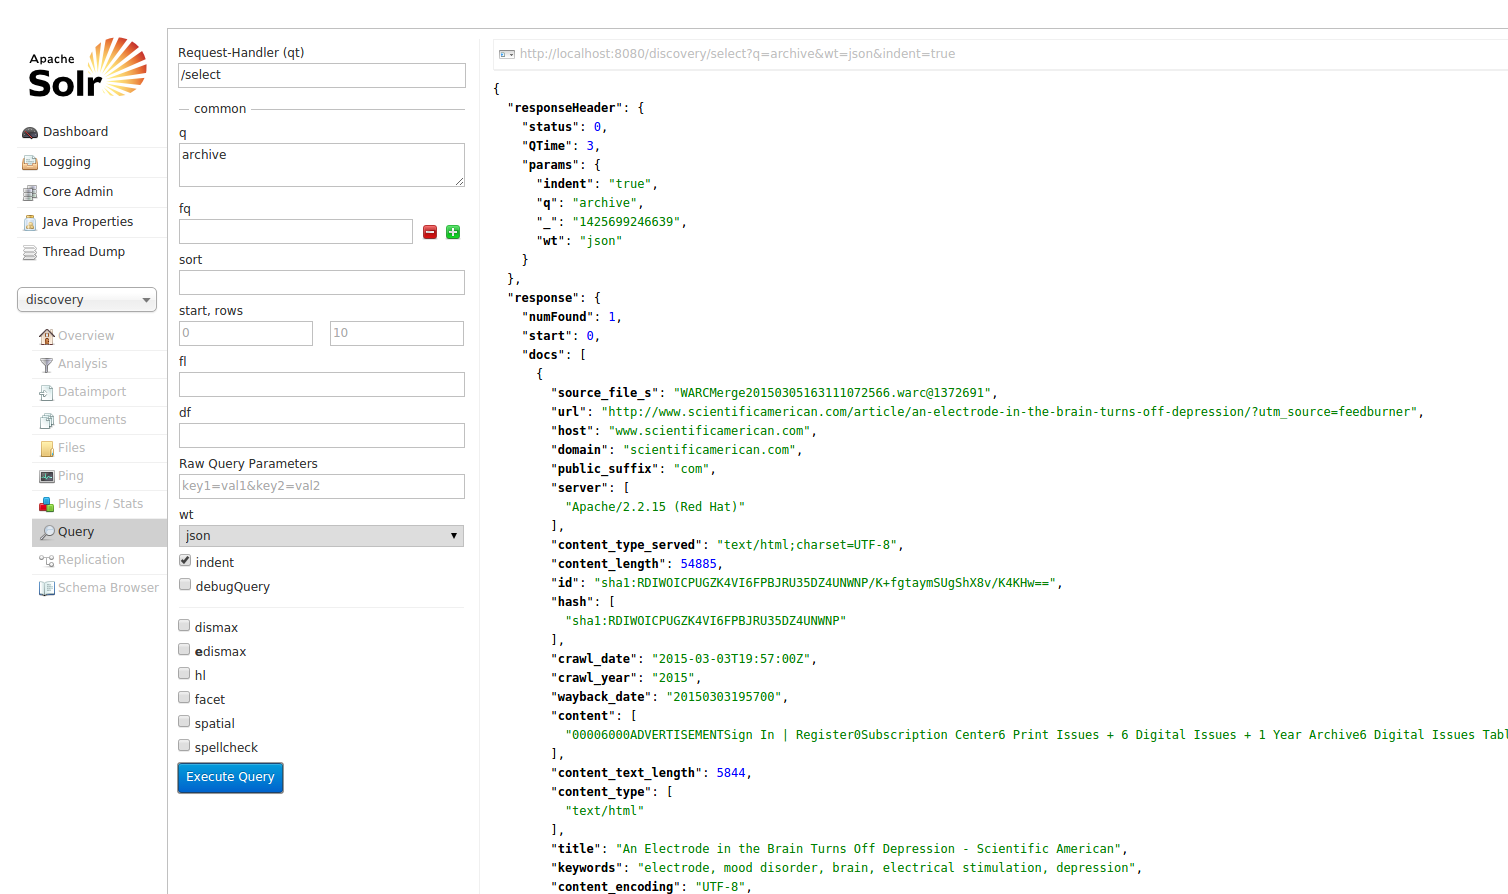
\includegraphics[scale=0.40]{query1.png}
		\caption{Query 1 on SOLR}
		\end{center}
\end{figure}	
\begin{figure}[ht]
	\begin{center}
		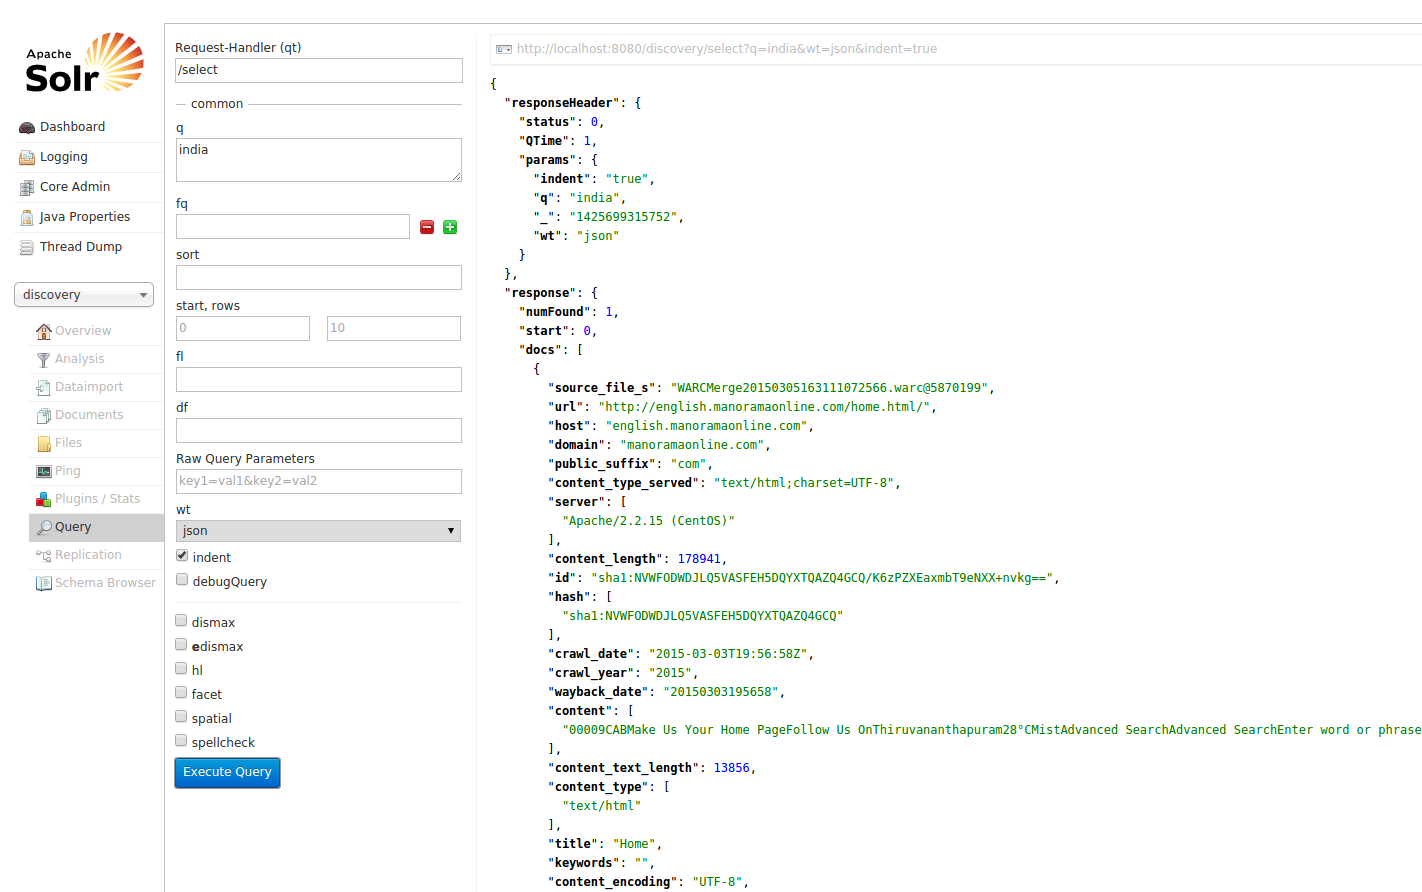
\includegraphics[scale=0.40]{query2.png}
		\caption{Query 2 on SOLR}
		\end{center}
\end{figure}
\begin{figure}[ht]
	\begin{center}
		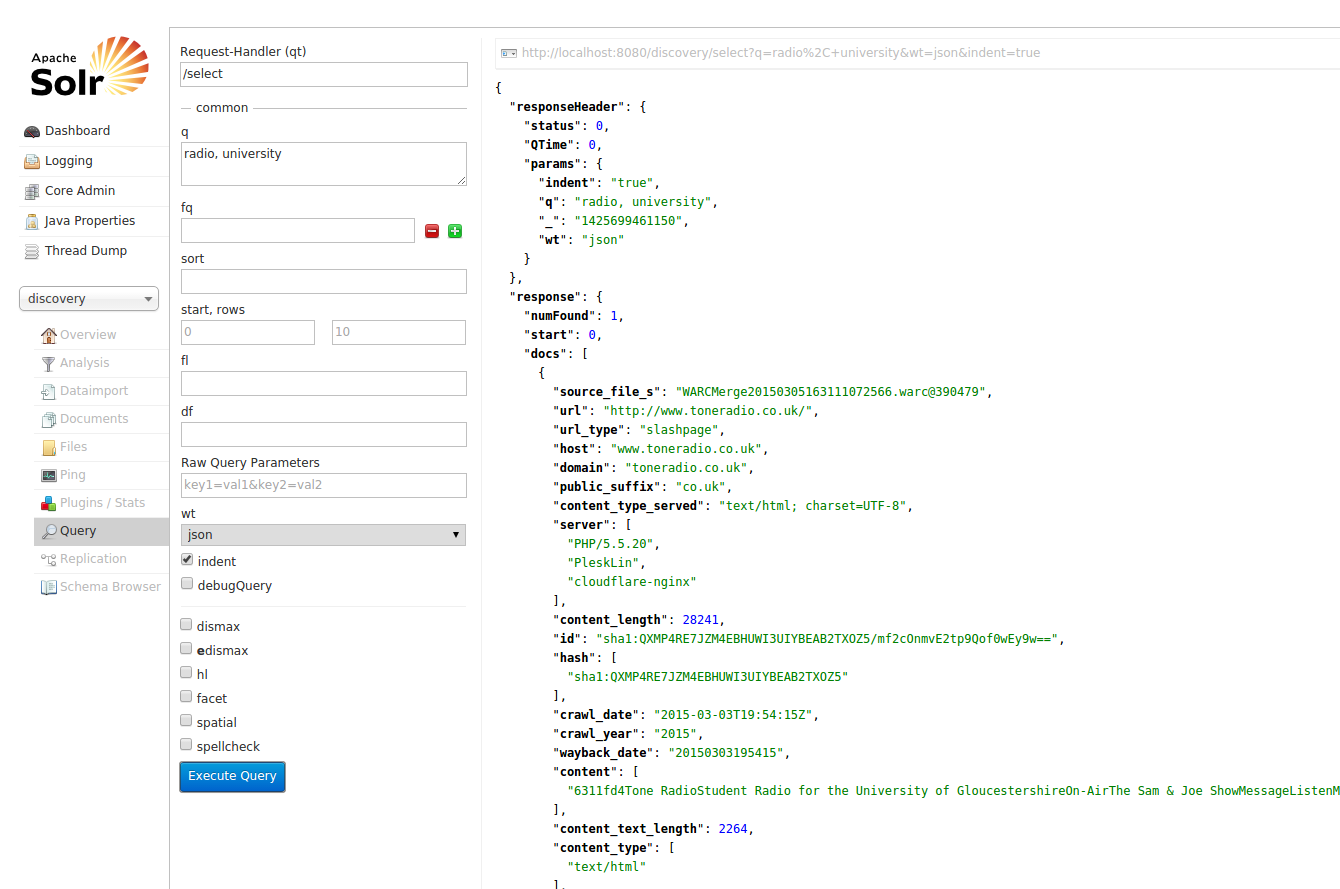
\includegraphics[scale=0.40]{query3.png}
		\caption{Query 3 on SOLR}
		\end{center}
\end{figure}
\newpage